% !TeX program = xelatex
% !TeX root = RP1_ICSMD2026_English_Revised_R1.tex
% !BIB program = bibtex
% !TeX encoding = UTF-8
\documentclass[conference,a4paper]{IEEEtran}

% ICSMD 2026: A4, two-column IEEE conference layout, 5--6 pages.
\usepackage{fontspec}
\setmainfont{Times New Roman}
\setsansfont{Arial}
\setmonofont{Consolas}

\usepackage{amsmath,amssymb}
\usepackage{graphicx}
\usepackage{booktabs}
\usepackage{array}
\usepackage{tabularx}
\usepackage{multirow}
\usepackage{url}
\usepackage{xurl}
\usepackage{cite}
% R1: yellow highlighting is enabled by default. Define \CleanVersion to hide it.
\usepackage[table]{xcolor}
\usepackage{soul}
\sethlcolor{yellow!40}
\DeclareRobustCommand{\rev}[1]{\ifdefined\CleanVersion#1\else\hl{#1}\fi}
\soulregister\cite7
\soulregister\ref7
\soulregister\emph1
\soulregister\textbf1
\newcommand{\revtable}{\ifdefined\CleanVersion\else\rowcolors{1}{yellow!25}{yellow!25}\fi}
\definecolor{revisionfigure}{RGB}{255,255,224}
\ifdefined\CleanVersion\colorlet{revisionfigure}{white}\fi
\usepackage{pgfplots}
\usepackage{balance}
\usepackage{needspace}
\usepackage{float}
\usepackage{microtype}
\pgfplotsset{compat=1.18}

\IEEEoverridecommandlockouts

\setlength{\columnsep}{0.24in}
\setlength{\textfloatsep}{5pt plus 1pt minus 1pt}
\setlength{\floatsep}{4pt plus 1pt minus 1pt}
\setlength{\intextsep}{4pt plus 1pt minus 1pt}
\setlength{\abovecaptionskip}{3pt}
\setlength{\belowcaptionskip}{0pt}
\renewcommand{\arraystretch}{1.08}

\title{Evidence-Traceable Knowledge Graph Construction from Marine Pump Technical Documents via Automated Evidence-Quality Gating}

\author{%
\IEEEauthorblockN{Xiaokun Zhang\textsuperscript{1}, Dongliang Fu\textsuperscript{1,*}, Rui Wang\textsuperscript{2}, and Erwu Liu\textsuperscript{2}}
\IEEEauthorblockA{\textsuperscript{1}Shanghai Marine Equipment Research Institute (SMERI), China State Shipbuilding Corporation (CSSC), Shanghai, China\\
\textsuperscript{2}Tongji University, Shanghai, China\\
\textsuperscript{*}Corresponding author: Dongliang Fu; e-mail: fdl@163.com}}

\begin{document}
\maketitle

\begin{abstract}
Measurements from marine engine-room pumps become more interpretable and auditable when linked to documented causes, inspections, and maintenance actions. Large language models can extract such relations from manuals, but their outputs may contain unlocatable evidence, reversed relations, misaligned table cells, or duplicated support copied across documents. This paper presents an automated evidence-quality gating method for constructing a page-traceable and auditable knowledge graph. Each normalized triple is stored separately from every page-level evidence record that supports it. Admission requires valid graph structure and direction, recoverable page or table evidence, relation support, complete provenance, build-corpus membership, and non-inference. A full audit graph retains all candidates and gate outcomes; evidence-qualified records with normalized Chinese terminology form tiered application graphs. From 15 documents and 1,934 physical pages, the pipeline produced 8,003 audit records, of which 1,698 passed all evidence gates. \rev{The standard application layer contains 1,326 evidence records and 1,281 unique triples, covering 78.09\% of the evidence-qualified set. On 20 fixed pages, complete gating retained 148 records with both endpoints recoverable inside the located evidence, compared with 223 of 243 records retained by simple filtering of the same candidates.} \rev{All 1,698 evidence-qualified records passed re-localization and provenance checks; all 13,729 controlled rule violations triggered a gate. Four held-out documents from one source family yielded 81 records meeting the non-corpus evidence gates.} Eightfold replication within one source family did not change the family-capped support score. The method enables evidence-grounded graph construction without manual approval of every triple at admission time. Qualification denotes compliance with declared evidence rules, not expert-confirmed factual or diagnostic accuracy.
\end{abstract}

\begin{IEEEkeywords}
marine pump systems, knowledge graph, evidence-quality gating, page-level provenance, terminology normalization, condition-monitoring knowledge
\end{IEEEkeywords}

\section{Introduction}

Pumps, motors, pipes, and valves in a ship's engine room support cooling, ballast transfer, bilge drainage, and fuel delivery. Condition-monitoring systems observe insufficient inlet pressure, reduced flow, elevated vibration, high temperature, and abnormal current \cite{ABS2016,ABS2023}. These measurements seldom identify a fault alone; engineers consult classification guidance, manuals, and maintenance tables to link them to possible causes and actions.

Such knowledge is evidence-dependent. A relation may appear in prose, a troubleshooting table, or a maintenance procedure; tables may contain merged rows and inherited headers. Retaining only a deduplicated head--relation--tail triple loses the exact supporting passage. Moreover, manuals from one source often repeat content, so document count overstates independent support.

Knowledge graphs organize equipment, faults, symptoms, inspections, and maintenance actions \cite{Hogan2021,Ji2022}. LLMs reduce extraction effort, but schema alignment, canonicalization, and output stability still require explicit controls \cite{Zhang2024EDC}. Industrial fault graphs mainly address extraction, fusion, reasoning, or diagnosis \cite{Han2022,Cai2024,Wu2024}. A preceding issue remains: what document-evidence conditions should an automatically extracted record satisfy before entering an application graph?

We treat each generated triple as a candidate, not a fact. It must point to recoverable evidence and pass frozen executable checks for field completeness, structure, direction, localization, provenance, and corpus boundaries. Passing denotes compliance with these admission rules, not expert confirmation of objective truth.

The study asks whether the pipeline produces schema-compliant, page-localized, provenance-complete records (RQ1); \rev{how evidence and terminology gates affect record retention and graph size (RQ2)}; whether frozen rules transfer to held-out sources (RQ3); whether source-family capping resists within-family duplication (RQ4); and how terminology tiers affect predefined fault-path coverage and density (RQ5).

The contributions are threefold. First, normalized triples are separated from page-level evidence records, preserving multiple supports after semantic deduplication. Second, executable gates jointly determine qualification, quarantine, or rejection and retain a complete audit trail. Third, tiered Chinese application graphs are derived from the audit graph, while source-family capping limits repeated documents assigned to one family from appearing as independent corroboration. We evaluate these mechanisms by complete-candidate re-audit, controlled fault injection, terminology sensitivity, source holdout, and replication stress tests.

\section{Related Work}

\subsection{LLM-Based Knowledge Graph Construction}

Knowledge graph construction combines extraction, schema alignment, canonicalization, and fusion \cite{Hogan2021,Ji2022}. Extract-Define-Canonicalize separates open extraction, schema definition, and post-hoc canonicalization, showing why LLM construction is not a single prompting step \cite{Zhang2024EDC}. Industrial graphs support process monitoring, rotating machinery, and equipment diagnosis \cite{Han2022,Cai2024,Wu2024}. Our focus is earlier: the evidence requirements that generated records must meet when manual review of every triple is not a prerequisite.

\subsection{Statement-Level Provenance and Evidence Support}

W3C PROV-O represents derivation through entities, activities, and agents \cite{W3CPROVO}; named or contextualized graphs can retain statement-level provenance \cite{Sikos2020}. RDF 1.2 triple terms and reifiers describe a statement without directly asserting it \cite{W3CRDF12}, while nanopublications separate an assertion from provenance and publication information \cite{Groth2010}. ProVe verifies textual support for graph triples \cite{Amaral2024ProVe}; SciGraph-LLM jointly extracts atomic claims, source spans, and provenance \cite{Malashin2026}.

Marine documents add physical-page and table localization, directed relations, Chinese terminology, and repeated content within source families. Rather than proposing a provenance standard, we turn established representation principles into an executable admission workflow.

\section{Method}

\subsection{Corpus Partition and Page Parsing}

MP numbers are corpus registry IDs, not a continuous build-set sequence. The build set comprises MP001--MP007 and MP015--MP022: 15 documents and 1,934 physical pages. \rev{MP008 supported parser, prompt, and rule debugging; its two retained pilot candidates do not establish statistical parameter calibration. MP009 was screened before the split and provides only a non-blind transfer case. MP010--MP013 were first processed after method and graph freezing, without feedback into parameter selection. MP008--MP013 remain outside the primary graph.} MP014 was excluded because it is an offshore electric-submersible-pump signal dataset rather than a marine technical document.

Deterministic rules removed blank, cover/title, contents, index, and exact-duplicate pages, leaving 1,889 extraction pages. Each page object retained text, table cells, bounding boxes, physical page, URL, publisher, source family, and document/page hashes. Candidate generation used the Alibaba Cloud Model Studio alias \mbox{qwen3.7-max} through the DashScope API at temperature zero on July 26--27, 2026; requests and responses were cached. The API records contain the alias rather than a dated model snapshot, so the historical backend snapshot cannot be established retrospectively.

The schema contains 13 node and 15 relation types. \rev{Types, directions, the whitelist, source families, and thresholds were frozen before holdout processing. Build-set results are not independent of earlier iterative rule design. Terminology experiments and the revision's parameter perturbations retain frozen evidence decisions and select no replacement settings.}

\subsection{Normalized Triples and Page-Level Evidence Records}

A normalized triple is denoted by
\begin{equation}
c_i=(h_i,r_i,t_i),
\label{eq:triple}
\end{equation}
where $h_i$, $r_i$, and $t_i$ are the head entity, relation, and tail entity. Every occurrence of document support creates a separate page-level evidence record:
\begin{equation}
a_i=\langle c_i,e_i,p_i,g_i\rangle,
\label{eq:evidence}
\end{equation}
\rev{Page-level evidence ($e_i$) is the supporting passage or table cells; page-level provenance ($p_i$) records document identity, physical page, URL, publisher, source family, and hashes.} The component $g_i$ stores evidence type, support mode, score, and gate outcomes. A triple may link to multiple evidence records; semantic deduplication never overwrites page-level support.

For example, MP016 p.~3 states that insufficient inlet pressure causes pump cavitation. The model proposes \emph{insufficient inlet pressure--causes--cavitation}. The system validates its types and direction, relocates both endpoints and the relation phrase, and stores page, URL, hashes, and source family. A repeated sentence in another manual adds evidence but not another contribution from that family.

\subsection{Automated Evidence-Quality Gating}

The gates comprise four groups.

\textbf{Structure:} Endpoint types, relation, and direction must comply with the whitelist and schema.

\textbf{Evidence:} E1 requires both entities in one continuous page span. \rev{E2 requires relevant cells in one row or validated merged-row group, resolvable cell locations, column names, and an affirmative layout-validation flag. Re-localizing cell coordinates alone does not satisfy all E2 admission conditions.} Cross-sentence E3 records remain auditable but cannot enter an application graph.

\textbf{Relation support:} Explicit rules require an unambiguous phrase or table role. Otherwise, the extraction model receives support- and rejection-oriented prompts. Both must support the relation at confidence $\geq0.9$, with relocatable quotations.

\textbf{Admission boundary:} The governance score $q_i=\alpha_i w_E(l_i)w_R(\eta_i)$ combines model-reported confidence $\alpha_i$ with frozen weights for evidence level and relation-support status. The weights for E1/E2/E3 are 1.00/0.95/0.75, and those for supported/undetermined/unsupported relations are 1.00/0.75/0. A record must belong to the build set, be non-inferred, contain complete URL/family/hash provenance, and have $q_i\geq0.8$. This heuristic supports filtering; it is not a factual probability.

\rev{The weights express a heuristic ordering, not calibrated probabilities: E1 and supported relations provide the unit reference, E2 receives a small alignment penalty, and reconstructed or unresolved support is discounted. No expert calibration or optimization search is documented. The 0.80 threshold requires confidence of at least 0.80 for E1 and approximately 0.8421 for E2, after mandatory evidence checks. Section IV-C examines sensitivity.}

The combined gate is
\begin{equation}
H(a_i)=I_{str}I_{dir}I_{loc}I_{sup}I_{prov}I_{build}I_{noninf}I_{q\geq0.8}.
\label{eq:gate}
\end{equation}
\rev{All indicators must equal one for evidence qualification. E3 and unresolved relations cannot qualify regardless of their weights. Recoverable cases enter quarantine if their final or applicable structural score reaches the separate 0.60 candidate floor; fatal failures or lower scores cause rejection. This floor differs from the 0.80 admission threshold.}

\begin{figure*}[t]
  \centering
  \IfFileExists{RP1_ICSMD2026_method_flowchart_en.pdf}{%
    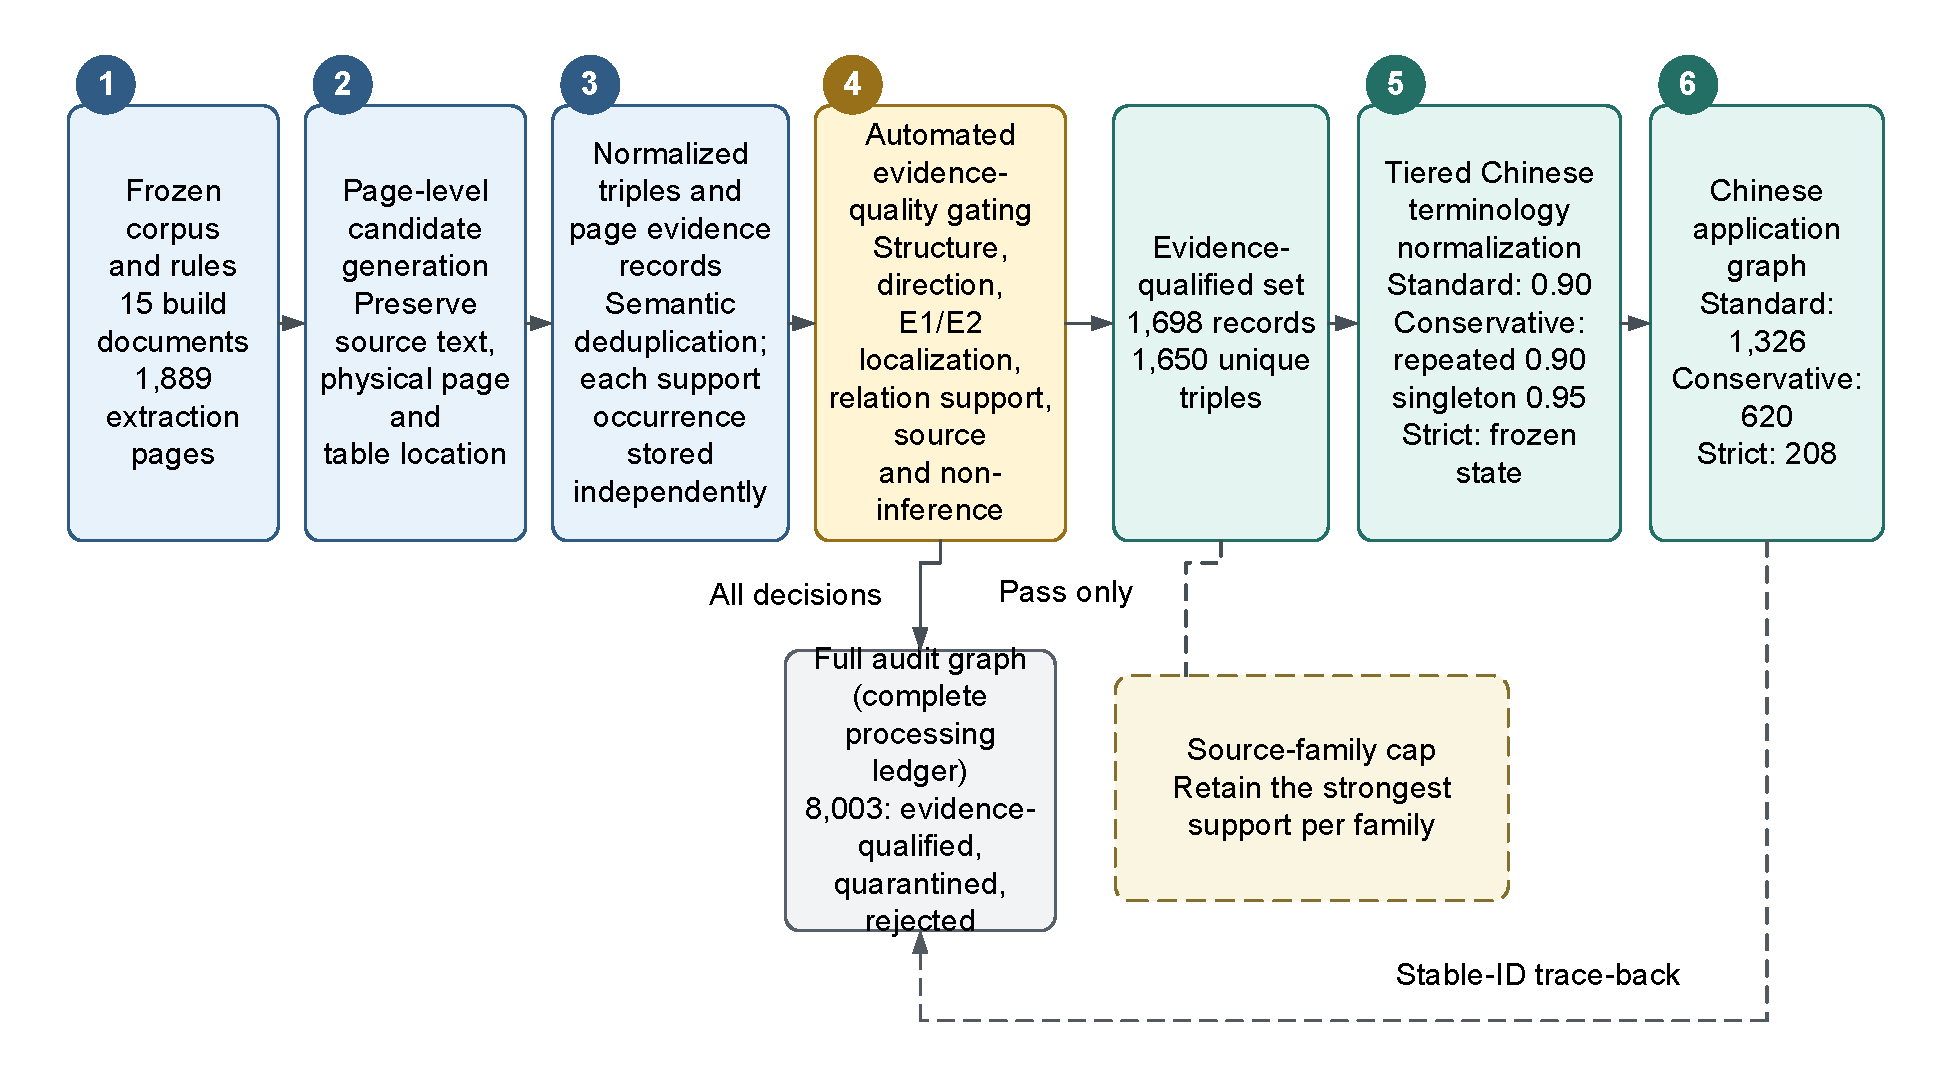
\includegraphics[width=0.90\textwidth]{RP1_ICSMD2026_method_flowchart_en.pdf}%
  }{\fbox{\parbox[c][35mm][c]{0.94\textwidth}{\centering Export the English workflow from the Visio source in this directory.}}}
  \caption{Workflow for automated evidence-quality gating, the complete processing ledger, and tiered Chinese application graphs.}
  \label{fig:pipeline}
\end{figure*}

\subsection{Full Audit Graph and Tiered Chinese Application Graphs}

The \emph{full audit graph} retains every candidate, gate outcome, and failure reason. The \emph{Chinese application graph} selects \rev{evidence-qualified}, non-inferred records for retrieval and visualization, then assigns standard, conservative, or strict layers from both endpoints' terminology status. Stable IDs link each application record to the audit graph and physical page (Fig.~\ref{fig:pipeline}).

Normalization never rewrites verbatim evidence. Frozen dictionary and earlier two-prompt terms are retained. Other Chinese names require completeness, no same-type naming conflict, protected-string preservation, and the layer threshold. Standard uses 0.90; conservative uses 0.90 for recurring endpoints and 0.95 for singletons; strict retains only the original frozen status. Protected strings include models, units, API, ISO, and NPSH. These checks indicate local consistency, not independent or expert confirmation.

\subsection{Source-Family Capping}

Manuals from one publisher may share content. For triple $c$, only the strongest evidence score in each publisher- or document-defined family is retained:
\begin{equation}
s_f(c)=\max_{a_i\in A_f(c)}q_i,\quad
S_{fam}^{(B)}(c)=\frac{1}{B}\sum_{j=1}^{\min(B,|F_c|)}s_{(j)}(c).
\label{eq:family}
\end{equation}
Here $F_c$ is the set of families supporting $c$, $s_{(j)}$ is the $j$th-largest family score, and $B=2$ is the frozen engineering coverage target; missing family slots contribute zero. The index is audit and ranking metadata and does not change gate decisions or application-graph membership. Duplicates within one family therefore cannot increase its contribution. The family label is an engineering proxy for dependence, not proof of independence.

\section{Experiments and Results}

\subsection{Experimental Setup}

\rev{Evaluation covered full-corpus gating, re-audit, fault injection, fixed-page baselines, terminology layers, parameter sensitivity, source holdout, replication, and fault paths. The revision analyses reused frozen candidates and cached responses, made no API calls, and verified that input hashes were unchanged. No human factual labels were available.}

\begin{table}[t]
\caption{Page Localization and Provenance Re-Audit}
\label{tab:audit}
\centering
\footnotesize
\setlength{\tabcolsep}{3.2pt}
\begin{tabular}{lrrrr}
\toprule
Decision & Records & Evidence & Endpoints & Subchecks \\
\midrule
\rev{Evidence-qualified} & 1698 & 100.00\% & 100.00\% & 100.00\% \\
Quarantined & 881  & 100.00\% & 100.00\% & 62.54\% \\
Rejected    & 5424 & 72.77\%  & 48.80\%  & 31.47\% \\
\bottomrule
\end{tabular}
\end{table}

\begin{table}[t]
\caption{Controlled Fault-Injection Results}
\label{tab:mutation}
\centering
\footnotesize
\setlength{\tabcolsep}{3.0pt}
\begin{tabular}{llrr}
\toprule
Fault group & Corrupted fields & Cases & Detection \\
\midrule
Identity/provenance & hash, URL, family & 6792 & 100.00\% \\
Page/evidence       & page, span, endpoints & 4943 & 100.00\% \\
Structural type     & relation-tail type & 1698 & 100.00\% \\
Table structure     & cell ID, bounding box & 296 & 100.00\% \\
\midrule
Total & 10 fault types & 13729 & 100.00\% \\
\bottomrule
\end{tabular}
\end{table}

\begin{table*}[!t]
\caption{Effect of Chinese Terminology Layers on Application-Graph Size and Fault-Path Density}
\label{tab:tiers}
\centering
\footnotesize
\setlength{\tabcolsep}{3.5pt}
\begin{tabularx}{\textwidth}{l>{\raggedright\arraybackslash}Xrrrrrr}
\toprule
Layer & Terminology rule & Evidence & Unique & Chinese & Path & Mean & Mean \\
      &                  & records  & triples & entities & coverage & answers & evidence \\
\midrule
Strict & Frozen dictionary and two-prompt status & 208  & 203  & 281  & 34/40 & 5.075 & 6.150 \\
Conservative & Recurring 0.90; singleton 0.95 & 620  & 590  & 870  & 34/40 & 5.575 & 6.800 \\
Standard & Uniform threshold of 0.90 & 1326 & 1281 & 2022 & 34/40 & 6.400 & 7.700 \\
\bottomrule
\end{tabularx}
\end{table*}

\begin{table}[!t]
\caption{\rev{Simple Baselines and Gating on the Same 20 Pages}}
\label{tab:prompt}
\centering
\footnotesize
\setlength{\tabcolsep}{3pt}
\revtable
\begin{tabular}{lrrr}
\toprule
Configuration & Records & Evidence & Both endpoints \\
\midrule
Direct LLM & 162 & 45.06\% & 40.12\% \\
Direct LLM + basic & 115 & 61.74\% & 56.52\% \\
\midrule
Shared: no gate & 367 & 87.74\% & 79.56\% \\
Shared: basic & 243 & 97.94\% & 91.77\% \\
Shared: full & 148 & 100.00\% & 100.00\% \\
\bottomrule
\end{tabular}
\end{table}

\subsection{Complete Candidate Re-Audit and Controlled Fault Injection}

The 8,003 records referenced 922 physical pages. Without reading original decision labels, re-audit reloaded page objects and checked document-page mappings, hashes, URLs, publishers, families, evidence and endpoint spans, and E2 table locations.

Table~\ref{tab:audit} shows that all 1,698 \rev{evidence-qualified} records passed localization, provenance, and type checks. All 881 quarantined records retained locatable evidence and endpoints; 330 failed the listed subchecks because they used E3 reconstruction. Of 5,424 rejected records, 3,947 retained locatable evidence, 2,647 both endpoints, and 1,707 all listed subchecks. \rev{Of those 1,707, 1,451 still failed original E2 admission requirements: 1,449 lacked the affirmative layout flag and 290 lacked column names, with overlap. A further 253 failed relation support and three fell below the 0.60 candidate floor. The re-audit checks recoverability, but does not replace these recorded admission requirements.}

\rev{Table V assigns each rejection to its first failed category in the stated order, not to a gate's independent causal effect. Flags overlap: 4,632 records have evidence failures and 2,777 have rule-based relation-support failures.}

\begin{table}[t]
\caption{\rev{Primary Failure Categories Among Rejected Records}}
\label{tab:rejections}
\centering\footnotesize
\revtable
\begin{tabular}{lrr}
\toprule
Attribution order and category & Records & Share \\
\midrule
1. Schema/type incompatibility & 1292 & 23.82\% \\
2. Evidence admission failure & 3868 & 71.31\% \\
3. Relation support failure & 253 & 4.66\% \\
4. Below 0.60 candidate floor & 11 & 0.20\% \\
\midrule
Total & 5424 & 100.00\% \\
\bottomrule
\end{tabular}
\end{table}

Fault injection corrupted one declared rule at a time in the 1,698 \rev{evidence-qualified} records. Ten fault types covered identity/provenance, page/evidence location, endpoint types, and tables. Every valid mutation triggered a gate (Table~\ref{tab:mutation}); this tests encoded-rule response, not general semantic-error detection.

\subsection{Full-Corpus Graph, Terminology Layers, and Gate Contributions}

From 8,071 raw candidates, normalization and deduplication produced 8,003 audit records: 1,698 \rev{evidence-qualified}, 881 quarantined, and 5,424 rejected. \rev{The evidence-qualified records} represent 1,650 unique triples and 2,613 source-language entities.

By relation-support mode, explicit phrases supported 784 records and table roles supported 98; the other 816 used same-model two-prompt consistency and were marked separately because it is not independent validation. By evidence-localization mode, the \rev{evidence-qualified} set comprised 1,550 E1 and 148 E2 records.

\rev{Before score filtering, 1,704 records met the remaining hard gates; 1,698 passed the 0.80 threshold. This six-record reduction concerns admission, whereas Table V concerns the separate rejected-record population.}

\rev{Terminology processing kept all evidence decisions fixed (Table III). The standard layer covers 78.09\%, with 6.38 times as many records as strict. Its 372 exclusions involve 286 unresolved endpoint groups: 205 below 0.90 confidence, 75 with missing or conflicting Chinese names, and six failing protected-string preservation. Endpoints recur, and either endpoint can block a record.}

\rev{MP003, MP005, and MP022 contribute 149, 74, and 39 exclusions, with within-document rates of 29.04\%, 27.82\%, and 40.21\%. Maintenance, inspection, and prevention relations contribute 118, 84, and 58 exclusions, with rates of 25.99\%, 22.40\%, and 34.32\%. The longer endpoint has a median of nine words among excluded records, versus seven among included records. Lowering only the terminology threshold to 0.88 or 0.85 would admit 1,329 or 1,491 records. These uneven losses expose a coverage cost; without semantic labels, they neither establish the additional names' correctness nor rule out overfitting.}

\rev{Both expanded layers passed 36 release checks covering integrity, IDs, evidence links, splits, evidence types, provenance, schema, terminology, and verbatim preservation. A non-blocking warning concerned 40 rejected records lacking verbatim text. Evidence and terminology thresholds govern separate decisions.}

\rev{A joint sweep on 1,704 hard-gate survivors crossed four E2 weights (0.85, 0.90, 0.95, 1.00), three supported-relation weights (0.90, 0.95, 1.00), and seven thresholds (0.75, 0.80, 0.85, 0.90, 0.925, 0.95, 0.975): 84 combinations. At threshold 0.80, counts range from 1,398 to 1,698. With support weight 1.00, E2 weights of 0.90--1.00 retain 1,697--1,698 records. At E2 weight 0.95, support weights of 0.95 and 0.90 retain 1,678 and 1,525. E3 and undetermined weights cannot affect admission under their hard vetoes.}

\rev{Figure 2 shows the joint sensitivity. Original weights retain 1,698 records at 0.80 but only 36 at 0.975. Higher thresholds expose clustered confidence values. The post-submission sweep describes sensitivity, not optimality or a historical parameter-selection procedure.}

\begin{figure}[t]
\centering
\colorbox{revisionfigure}{%
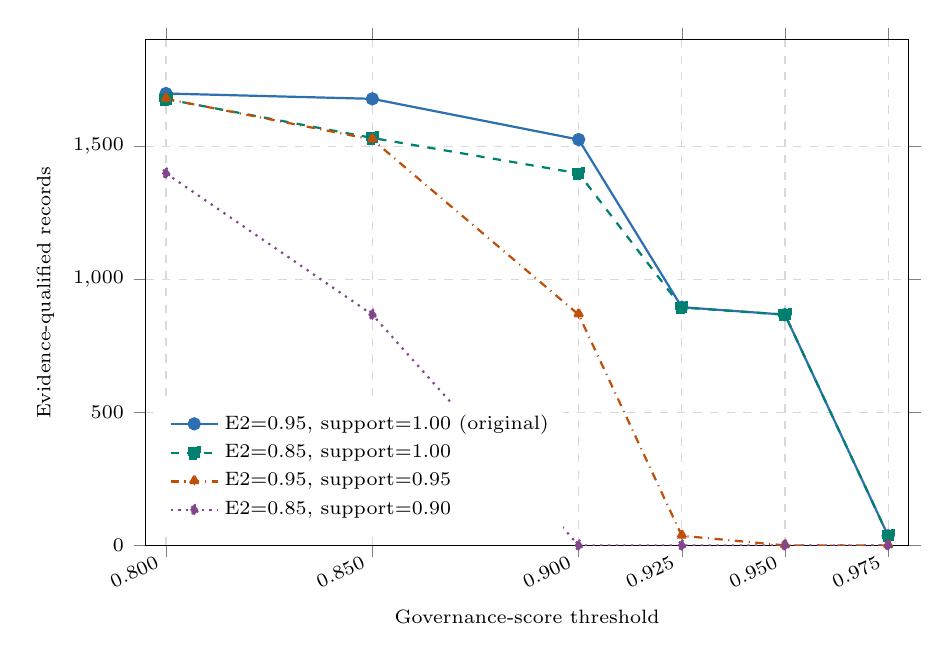
\begin{tikzpicture}
\begin{axis}[
  width=0.93\columnwidth,
  height=0.66\columnwidth,
  xlabel={Governance-score threshold},
  ylabel={Evidence-qualified records},
  xmin=0.795, xmax=0.980,
  ymin=0, ymax=1900,
  xtick={0.800,0.850,0.900,0.925,0.950,0.975},
  xticklabel style={font=\scriptsize,rotate=25,anchor=east,/pgf/number format/fixed,/pgf/number format/precision=3,/pgf/number format/zerofill},
  yticklabel style={font=\scriptsize},
  label style={font=\scriptsize},
  grid=major,
  grid style={draw=gray!30,dashed},
  axis line style={black},
  tick align=outside,
  legend style={font=\scriptsize,at={(0.02,0.03)},anchor=south west,fill=white,draw=none},
  legend cell align={left},
]
\addplot[color={rgb,255:red,45;green,111;blue,176},mark=*,thick]
coordinates {(0.800,1698) (0.850,1678) (0.900,1525) (0.925,895) (0.950,867) (0.975,36)};
\addlegendentry{E2=0.95, support=1.00 (original)}
% Exact revision sweep values are inserted below after analysis.
% Generated values: revision_r1_20260905/weight_threshold_sensitivity.csv.
\addplot[color={rgb,255:red,0;green,128;blue,110},mark=square*,dashed,thick]
coordinates {(0.800,1677) (0.850,1531) (0.900,1398) (0.925,894) (0.950,867) (0.975,36)};
\addlegendentry{E2=0.85, support=1.00}
\addplot[color={rgb,255:red,190;green,80;blue,10},mark=triangle*,dashdotted,thick]
coordinates {(0.800,1678) (0.850,1525) (0.900,867) (0.925,36) (0.950,0) (0.975,0)};
\addlegendentry{E2=0.95, support=0.95}
\addplot[color={rgb,255:red,130;green,70;blue,140},mark=diamond*,dotted,thick]
coordinates {(0.800,1398) (0.850,867) (0.900,0) (0.925,0) (0.950,0) (0.975,0)};
\addlegendentry{E2=0.85, support=0.90}

\end{axis}
\end{tikzpicture}}
\caption{\rev{Joint weight and threshold sensitivity with all hard gates fixed.}}
\label{fig:threshold}
\end{figure}

\subsection{\rev{Simple Baselines and Prompt-Rule Ablation}}

\rev{Table IV uses the original 20 evidence-rich build pages. Basic filtering requires nonempty triple and type fields, matches both endpoints anywhere on the page after case/whitespace normalization, and deduplicates within-page triples. It uses no evidence-span, table-alignment, relation-support, or score constraint. Direct LLM outputs keep their native schema. All rows use the same page/cell re-localizer; ``both endpoints'' requires both entities inside the located evidence.}

\rev{The lower three rows fix the full prompt's 367 normalized candidates. Basic filtering retains 243 records, with 223 (91.77\%) passing endpoint localization; full gating retains 148, all passing. Basic filtering retains only 98 of those 148: the remaining 50 are E2 records recoverable from cells but missed by flat-page matching. Thus basic filtering can retain poorly grounded records and omit recoverable table evidence. Parser-supplied provenance is complete in every row, not a comparative gain.}

\rev{Historical B0--B3 are prompt-rule ablations (unconstrained, schema, evidence, and direction/applicability), yielding 0/50/31/32 evidence-qualified records versus 148 for the full prompt. Unmatched candidate/token limits prevent claims of extraction superiority. The shared-candidate comparison isolates post-processing at fixed extraction cost; direct-LLM rows provide a workflow reference. Neither measures factual precision, recall, or F1.}

\subsection{Source Holdout, Within-Family Replication, and Fault Paths}

After freezing the method and primary graph, MP010--MP013 underwent first extraction in isolation. Their 103 physical pages (94 after exclusions) yielded 287 audit records. Of these, 81 met the non-corpus evidence gates with complete page localization and provenance but retained held-out status under the build-boundary rule. They did not feed back into tuning. All belong to the MAIB family, so this test covers structural and evidence-rule behavior on unseen documents, not source diversity or external factual accuracy.

Three triples occurred identically in two documents from one family. Replicating evidence one, two, four, and eight times left the mean capped index at 0.461058 (maximum change zero). Direct document accumulation raised the mean from 0.461877 to 0.922116 and the number scoring $\geq0.8$ from three to 1,650. Thus within-family duplication cannot increase capped support; no natural identical cross-family triple was available to test cross-family discrimination.

Every terminology layer covered 34/40 predefined fault paths (85\%); the four groups remained 7/10, 10/10, 7/10, and 10/10. From strict to standard, mean answers rose from 5.075 to 6.400, page evidence from 6.150 to 7.700, documents from 2.700 to 3.075, and families from 2.350 to 2.600. Expansion increased density, not path types; these are not question-answering or diagnostic accuracy.

\section{Discussion}

\subsection{Meaning of Qualification and the Human-Review Boundary}

\rev{Re-localization and controlled fault injection show that evidence qualification is a repeatable executable state. They do not establish factual correctness.}

\rev{Terminology relaxation expands the application graph from 208 to 1,326 records without changing evidence gates. Stricter naming policies have not been shown to improve factual accuracy or diagnostic safety.}

\rev{Reusable rules remove triple-by-triple expert approval as an admission prerequisite, but cannot make manuals infallible. Human judgment defines the rules; conflicts, safety-critical statements, and out-of-scope conditions still warrant targeted review.}

\subsection{Relation-Support Modes and Measurement Knowledge}

Explicit phrases or table roles support 882 records; 816 use two checks by the extraction model. Their errors may be correlated, so the modes are exposed rather than treated as equally independent. Safety-critical retrieval can prioritize explicit-rule records or target model-consistency records for review.

This work addresses the knowledge-data layer of measurement and diagnosis, not a new sensor or classifier. The graph links pressure, flow, vibration, temperature, and current observations to documented causes, inspections, and maintenance, with a page basis for every relation. It can support evidence retrieval, diagnostic assistance, and later GraphRAG systems; no sensor time series or fault-recognition accuracy is reported.

\subsection{Limitations}

\rev{The study evaluates evidence auditability rather than state-of-the-art extraction accuracy. No expert factual labels were available for precision, recall, or F1. Shared-model relation checks and terminology suggestions may have correlated errors. Fault injection tests encoded violations. The direct-extraction runs are not budget matched, whereas the shared-candidate control fixes extraction outputs and cost. Heuristic weights remain uncalibrated; the post-submission sweep measures sensitivity rather than optimality. Terminology exclusions vary by source and relation, so overfitting cannot be ruled out. Source-family testing lacks natural identical cross-family triples.}

\section{Conclusion}

\rev{Automated evidence-quality gating separates normalized triples from page support and preserves every admission decision. Fifteen marine pump documents yielded 8,003 audit records, 1,698 evidence-qualified records, and a standard application layer of 1,326 records. Compared with basic filtering of shared candidates, full gating raises the endpoint-recovery rate and retains table evidence missed by page-wide matching. Rejection attribution, terminology analysis, and parameter sweeps clarify the coverage costs. The graph supplies traceable knowledge for measurement interpretation; factual and diagnostic accuracy remain unevaluated.}

\section*{Acknowledgment and Declarations}

\textbf{Data availability:} Code, configurations, scripts, and releasable derived results will be released upon acceptance. Copyrighted PDFs will not be redistributed; source URLs are retained with the evidence records. \textbf{Funding:} This research received no external funding. \textbf{Conflict of interest:} The authors declare no conflict of interest. \textbf{Ethics:} No human participants, animals, or personal data were involved. \textbf{Generative AI:} The Alibaba Cloud Model Studio alias \mbox{qwen3.7-max} generated candidates, performed same-model relation checks, and suggested initial Chinese terms through the DashScope API on July 26--27, 2026. The API returned the alias rather than a dated snapshot; prompt versions, request identifiers, and responses were retained. Terminology expansion used local records only. Generative AI assisted English translation and language editing. The authors reviewed the manuscript and take responsibility for its content.

% Balance the final manuscript page before any appended response pages.
\balance
\bibliographystyle{IEEEtran}
\bibliography{RP1_ICSMD2026_references_v5}

\ifdefined\IncludeResponse
  \clearpage
  \nobalance
  \onecolumn
  % Shared response text: standalone article or appended to the revised manuscript.
% !TeX root = RP1_ICSMD2026_Revision_Package_R1.tex
\begingroup
\normalfont\fontsize{11}{14}\selectfont
\setlength{\parindent}{0pt}
\setlength{\parskip}{7pt}
\setlength{\emergencystretch}{2em}
\pagestyle{plain}
\newcommand{\responseitem}[2]{\par\Needspace{8\baselineskip}\bigskip\noindent\textbf{Comment #1. #2}\par\nopagebreak}
\begin{center}
{\Large\bfseries Response to Reviewers}\par
\medskip
ICSMD 2026 --- Submission 46\par
\textit{Evidence-Traceable Knowledge Graph Construction from Marine Pump Technical Documents via Automated Evidence-Quality Gating}
\end{center}

Dear Editor and Reviewers,

Thank you for reviewing our manuscript. We have added simple extraction and filtering baselines, a breakdown of rejection reasons, an analysis of terminology exclusions, and a joint weight--threshold sensitivity analysis. We have also clarified the development and evaluation sequence and standardized the terminology. Changes in the manuscript are highlighted in yellow. Section and table references below refer to the revised manuscript. The comments are summarized before each response.

The added analyses use the retained candidate records, page objects, and extraction caches. They do not require new model calls or change the frozen graph. We distinguish these revision analyses from the original parameter choices throughout the response.

\bigskip
{\large\bfseries Reviewer \#2}

\responseitem{2.1}{B0--B3 are author-defined ablations rather than established baselines. Add a simple LLM extraction and filtering baseline, or clarify the focus on auditability and engineering applicability.}

We agree that the original comparison did not isolate the benefit of post-extraction gating. Table IV now includes direct LLM extraction, direct extraction with basic filtering, and three controls that share exactly the same 367 normalized candidates. The last three controls use no gate, basic filtering, and complete gating, respectively. This keeps extraction outputs and extraction cost fixed when comparing the post-processing methods.

Basic filtering requires complete head, relation, tail, and type fields, matches both endpoint strings anywhere on the source page after case and whitespace normalization, and removes identical triples within the same page. It does not use evidence-span constraints, table alignment, relation-support decisions, or confidence scores. The direct extraction baseline retains its native types and relation names. We no longer represent its failure to match our whitelist as evidence that all its statements are wrong.

On the shared candidate set, basic filtering retains 243 records. Both endpoints are recoverable inside the located evidence for 223 of them (91.77\%). Complete gating retains 148 records, all of which pass this check. Basic filtering retains only 98 of these 148 evidence-qualified records. The other 50 use table evidence that can be resolved through cell locations but fails flat-page string matching. These results show both the limitations of page-wide matching and the practical value of table-aware evidence recovery. Parser-supplied provenance is complete in all configurations and is not presented as an advantage of gating.

Section IV-D now identifies B0--B3 as historical prompt-rule ablations. Section V-C states that the comparison evaluates evidence auditability and does not establish state-of-the-art extraction accuracy. For engineering use, the graph connects observations with documented causes and actions and lets a user inspect their page evidence. The baseline comparison supports this evidence-management role; a diagnosis-performance claim would require a separate evaluation.

\textbf{Changes:} Table IV; Section IV-D, ``Simple Baselines and Prompt-Rule Ablation''; Section V-C; abstract and conclusion.

\responseitem{2.2}{Explain the primary failure gates among the 5,424 rejected records, including those that retain locatable evidence and endpoints.}

Table V reports the following mutually exclusive attribution. We assign a record to the first failed category in the order shown, since a record can have several failure flags.

\begin{center}
\begin{tabular}{lrr}
\toprule
Primary failure category & Records & Share \\
\midrule
Schema/type incompatibility & 1,292 & 23.82\% \\
Evidence admission failure & 3,868 & 71.31\% \\
Relation support failure & 253 & 4.66\% \\
Below the 0.60 candidate floor & 11 & 0.20\% \\
\midrule
Total & 5,424 & 100.00\% \\
\bottomrule
\end{tabular}
\end{center}

The percentages may sum to 99.99\% after rounding. These are order-dependent primary reasons, not independent estimates of each gate's contribution. Across overlapping flags, 4,632 rejected records have an evidence failure and 2,777 have a rule-based relation-support failure; a further 253 have a failed two-prompt relation check.

Checking the 1,707 rejected records that pass all re-localization subchecks revealed an omission in our earlier explanation. Of these records, 1,451 still fail the original E2 admission conditions. Among that group, 1,449 lack an affirmative table-layout validation flag and 290 lack column names; the two counts overlap. Another 253 fail relation support and three fall below the candidate score floor. Recovering cell coordinates and endpoint text does not establish that the table layout and column semantics met the original admission rules. Section IV-B now gives this breakdown explicitly.

We also distinguish the 0.60 candidate floor, which can cause rejection, from the 0.80 evidence-admission threshold. The six-record loss at 0.80 is measured among the 1,704 records that pass the other hard gates; it is not the count of score-based rejections among all 5,424 rejected records.

\textbf{Changes:} Sections III-C and IV-B; new Table V; the gate-count paragraph in Section IV-C.

\clearpage
{\large\bfseries Reviewer \#3}

\responseitem{3.1}{Add a baseline LLM extraction method without gating on the same documents; report evidence qualification, evidence locatability, and factual accuracy if annotations are available.}

Table IV now includes the requested direct-extraction baseline and a simple-filtering variant on the same 20 pages. Direct extraction produces 162 records, of which 73 (45.06\%) have recoverable evidence and 65 (40.12\%) also have both endpoints inside that evidence. Basic filtering retains 115 records, with corresponding rates of 61.74\% and 56.52\%. These rows are assessed using the same re-localizer as the other configurations, without requiring their native schema to match our relation whitelist.

The table also provides a controlled comparison on the full prompt's 367 normalized candidates. The no-gate, basic-filter, and full-gate outputs contain 367, 243, and 148 records; 148, 98, and 148 of those records, respectively, have the frozen evidence-qualified status. This status is an internal compliance measure, so the main table reports the separate evidence and endpoint recovery rates rather than presenting qualification counts as factual accuracy.

No factual annotations are available, and we therefore do not report factual accuracy or F1. The manuscript retains that limit. B0--B3 are explicitly called prompt-rule ablations, and the original 2.96-fold yield comparison is no longer used to argue an advantage over existing extraction methods.

\textbf{Changes:} Table IV; Section IV-D; Section V-C.

\responseitem{3.2}{Analyze the 372 terminology exclusions by relation and source, and assess whether the normalization rules are too strict or overfitted.}

We traced the 372 excluded records to 286 unresolved endpoint groups. Of these groups, 205 are below the 0.90 translation-confidence threshold, 75 have missing or conflicting Chinese labels, and six fail protected-string preservation. Endpoint and record counts differ because an endpoint can occur in several records and either endpoint can block admission.

The exclusions are not evenly distributed. MP003, MP005, and MP022 contribute 149, 74, and 39 records. Relative to each document's evidence-qualified records, these are exclusion rates of 29.04\%, 27.82\%, and 40.21\%, respectively. Maintenance, inspection, and prevention relations contribute 118, 84, and 58 exclusions, with within-relation rates of 25.99\%, 22.40\%, and 34.32\%. We report both counts and rates so that large documents and frequent relations are not mistaken for unusually high-risk groups merely because they contain more records.

The median word count of the longer endpoint is nine for excluded records and seven for included records. This is consistent with a greater burden for longer action descriptions, although it does not show that length causes the failures. A threshold-only relaxation, keeping completeness, conflict, and protected-string rules fixed, would increase the application set from 1,326 records to 1,329 at 0.88 and 1,491 at 0.85.

We now acknowledge that the terminology rule limits coverage and affects sources and relations differently. Without independent semantic labels, we cannot determine how many of the newly admitted names would be correct or claim that overfitting has been ruled out. The analysis is reported as a coverage tradeoff, and the frozen application layers are unchanged.

\textbf{Changes:} Section IV-C, terminology-exclusion and threshold-relaxation paragraphs; Sections V-A and V-C.

\responseitem{3.3}{Standardize ``page-level evidence'' versus ``page-level provenance,'' and ``qualified'' versus ``evidence-qualified.''}

Section III-B now defines page-level evidence as the supporting passage or table cells. Page-level provenance refers to the source metadata: document identity, physical PDF page, URL, publisher, source family, and hashes. The terms are used for content and origin, respectively. Accepted records are called ``evidence-qualified records'' throughout the manuscript, including the abstract, tables, figure axis, discussion, and conclusion.

\textbf{Changes:} Section III-B and terminology edits throughout the manuscript.

\responseitem{3.4}{Clarify what was adjusted using MP008 and whether development or preliminary transfer checks could contaminate the holdout evaluation.}

We have made the sequence and its limits explicit. MP008 supported parser, prompt, and rule debugging. The retained pilot contains only two MP008 candidate records; it does not support a claim that weights or thresholds were selected through a statistical search on that document. The revised manuscript does not make such a claim.

MP009 was screened before the split and is described only as a non-blind transfer case. MP010--MP013 were first processed after the method and primary graph had been frozen. Their records remained outside the graph, and their results were not used to adjust the rules or thresholds. The new sensitivity calculations use the frozen build records and select no replacement parameters.

We distinguish two issues in the revision: iterative development can make rules specific to the development/build material, while holdout contamination would require using the holdout material to guide changes. The former remains a limitation. The documented processing sequence and split restrictions address the latter; they do not prove that the rules are free from overfitting.

\textbf{Changes:} Section III-A, ``Corpus Partition and Page Parsing''; Sections IV-A and V-C. The original holdout results in Section IV-E are retained.

\responseitem{3.5}{Explain the evidence and relation weights and the choice of the 0.80 inclusion threshold.}

The original settings were engineering choices. We found no retained grid-search or expert-calibration record that would justify describing them as optimized, and have stated this directly in Section III-C.

The weights encode an ordering: E1 evidence and supported relations provide the reference value of 1.00; E2 receives a small penalty for dependence on table alignment; reconstructed evidence and unresolved relations receive a discount in the audit ledger; unsupported relations receive zero. The values 0.95 and 0.75 specify the size of those heuristic penalties, rather than an estimated probability of correctness.

The 0.80 threshold is a permissive confidence floor applied after the hard evidence requirements. With the original weights, E1 records need model confidence of at least 0.80 and E2 records approximately 0.8421. The hard conditions already prevent E3 and unresolved relations from entering the evidence-qualified set, regardless of their numerical weights. This distinction was not sufficiently clear in the submitted version.

To assess the practical consequences, we added a post-submission sensitivity analysis rather than reconstructing an unsupported parameter-selection history. At threshold 0.80 and supported-relation weight 1.00, changing the E2 weight from 0.90 to 1.00 changes the retained count from 1,697 to 1,698. With the original E2 weight, reducing the supported-relation weight from 1.00 to 0.95 retains 1,678 records. Larger perturbations and higher thresholds produce substantial reductions, which are reported in Figure 2 and Section IV-C. These results describe sensitivity; they do not establish that 0.80 is optimal.

\textbf{Changes:} Section III-C, weight rationale and score boundaries; Section IV-C and revised Figure 2; Section V-C.

\responseitem{3.6}{Add sensitivity analysis for combinations of weights rather than a single threshold.}

We evaluated 84 combinations on the 1,704 records that satisfy all non-score hard gates. The grid crosses E2 weights of 0.85, 0.90, 0.95, and 1.00; supported-relation weights of 0.90, 0.95, and 1.00; and thresholds of 0.75, 0.80, 0.85, 0.90, 0.925, 0.95, and 0.975. E1 remains the unit reference. Figure 2 plots the original setting and three weight combinations; the table below gives all weight combinations at the original 0.80 threshold.

\begin{center}
\begin{tabular}{lrrr}
\toprule
& \multicolumn{3}{c}{Supported-relation weight} \\
E2 weight & 0.90 & 0.95 & 1.00 \\
\midrule
0.85 & 1398 & 1531 & 1677 \\
0.90 & 1398 & 1658 & 1697 \\
0.95 & 1525 & 1678 & 1698 \\
1.00 & 1545 & 1679 & 1698 \\
\bottomrule
\end{tabular}
\end{center}

At threshold 0.80, the grid retains 1,398--1,698 records. Small changes around the original weights have limited effects, but the combined penalties can remove many table records. The curves also show sharp losses at high thresholds because model confidence values cluster at a few levels. Changing the E3 or undetermined-relation weight cannot alter admission while their hard vetoes remain active; we state this property separately rather than treating those weights as effective admission parameters.

All perturbations are descriptive revision analyses on fixed build records. The original weights, thresholds, graph, and holdout evaluation remain unchanged.

\textbf{Changes:} Section IV-C; Figure 2; parameter limitations in Section V-C.

\medskip
Sincerely,\par
Xiaokun Zhang, Dongliang Fu, Rui Wang, and Erwu Liu\par
Corresponding author: Dongliang Fu, \texttt{fdl@163.com}
\endgroup

\fi
\end{document}
